\begin{figure}[htbp]
\centering
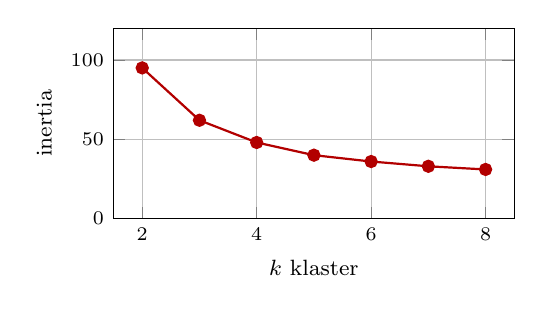
\begin{tikzpicture}
\begin{axis}[
  width=0.55\textwidth,
  height=4cm,
  xlabel={\footnotesize $k$ klaster},
  ylabel={\footnotesize inertia},
  xmin=1.5, xmax=8.5,
  ymin=0, ymax=120,
  grid=major,
  tick label style={font=\scriptsize}
]
\addplot[thick, red!70!black, mark=*] coordinates {
  (2,95) (3,62) (4,48) (5,40) (6,36) (7,33) (8,31)
};
\end{axis}
\end{tikzpicture}
\caption{Ilustrasi ``siku'' inertia vs $k$: penurunan melambat setelah suatu $k$; silhouette dapat dipakai sebagai kriteria tambahan.}
\end{figure}
